\chapter{Experiments}
\label{chapter:Experiments}

	This chapter presents implementation details of this work. Also datasets and evaluation measures used in this work are shown. The main part of this chapter presents the results of the clustering and feature selection components as well as results for the complete method.

	\section{Implementation}
	\label{sec:implemenation}

		All methods are implemented in Sun Java Version 6\footnote{\url{http://www.java.com/en/}}. As basic library \mbox{MULAN}\footnote{\url{http://mulan.sourceforge.net/}} is used \cite{mulan}. \mbox{MULAN} is a java library for multi-label learning based on the WEKA\footnote{\url{http://www.cs.waikato.ac.nz/~ml/weka/index.html}} machine learning software \cite{weka}.

		In figure \ref{img:classDiag} a class diagram of the implementation is shown. \textit{MultiLabelLearnerBase} is the base class for all multi-label learners within \mbox{MULAN}. For transformation-based learners, as described in section \ref{subsec:mlmethods}, an additional class called \textit{TransformationBasedMultiLabelLearner} provides additional parameters as the specification of a single label learner. \textit{TransformationBasedMultiLabelLearner} itself is a child of \textit{MultiLabelLearnerBase}. Methods presented in this work are placed into the \textit{TransformationBasedMultiLabelLearner} branch, as they transform the problem into smaller sub problems. The multi-label learner for both methods, CML and FCML, is called \textit{GroupBasedMetaClassifier}. It refers to a learner called \textit{FilteredMLLearner}, which acts as preprocessing step and filters the data by given feature and label subsets. \textit{FilteredMLLearner} forwards only the group containing the specified feature and label attributes to the actual learner. \mbox{MULAN} specifications enforce datasets to contain at least 2 labels, but groups with only one label may be used. Hence, an additional WEKA single label classifier is needed by \textit{FilteredMLLearner}.

		The class \textit{GroupBasedMetaClassifier} can use two classes for identifying groups: \textit{CML} and  \textit{FCML}. The classes implement the clustering based and feature selection and clustering based methods as described in section \ref{sec:CML} and \ref{sec:FCML}. The classes \textit{FMCL} and \textit{CML} identify groups and return them as indexes of attributes. These indexes are passed by \textit{GroupBasedMetaClassifier} to the \textit{FilteredMLLearner} class, which splits the dataset and forwards the subsets to the learner.

		By searching for labels not contained in a group, \textit{GroupBasedMetaClassifier} also ensures that the entire label space is covered. If labels are found which are not member of a group, an additional group is created, containing the missed labels and all features. Also, groups which do not contain a label will be ignored. Current methods only provide groups with disjoint label sets. Anyway, \textit{GroupBasedMetaClassifier} prediction method, can combine different votes for the same label. This is done by evaluating the "strongest" vote by the distance to an undetermined vote (confidence of $0.5$). \textit{GroupBasedLearner} also offers some methods for calculating statistics on datasets, like density or cardinality. All implementations provide full compatibility to \mbox{MULAN}.

		\begin{figure}
			\centering
			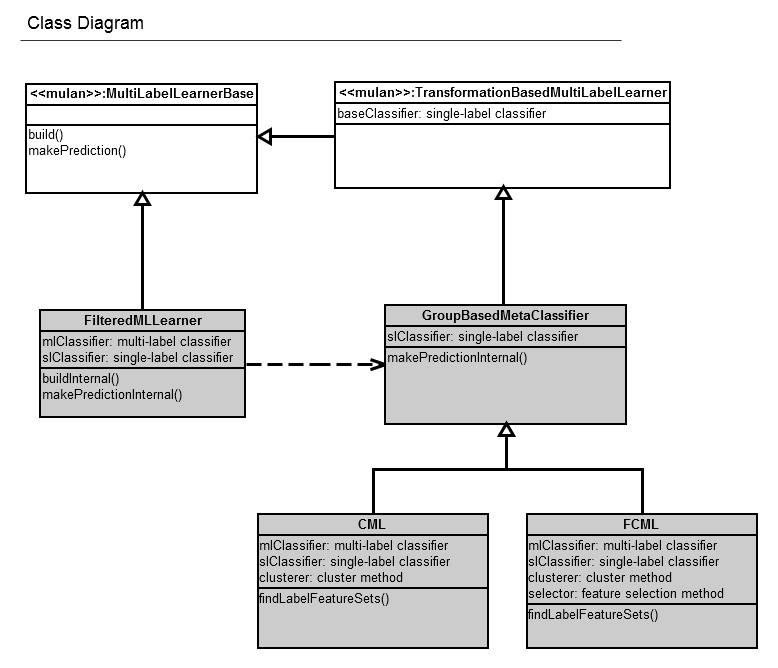
\includegraphics[width=\textwidth]{classdiagramm.png} 
			\caption{Class diagram showing the implementation structure of this work: self implemented classes are grey, white boxes represent \mbox{MULAN} classes. Most important input and output methods are shown. Drawn through lines indicate an "extends"-relationship, dashed lines an "used-by"-relationship.\newline Main class is the \textit{GroupBasedMetaClassifier} as it holds the subsets of the data "groups" and the multi-label classifier as well the single-label classifier. For every group a \textit{FilteredMLLearner} is used to extract the group subset from the dataset. For identifying groups either \textit{CML} or \textit{FCML} is used.}
		    \label{img:classDiag}
		\end{figure}

	\section{Multi-Label Datasets}
	\label{sec:datasets}

		A dataset can be described as $ N \times L \times M$ where $N$ is the number of instances, $ L $ the number of labels and $ M $ the number of features. \textit{Bibtex} and \textit{Delicious} are very large datasets in both label set cardinality and number of instances. This leads to very long computational times for clustering and feature selection. Therefore, those datasets where only tested with a small number of settings.

		In table \ref{tab:datasets} all datasets used in this work are presented. Additionally to their dimensions and type, the label cardinality ($LCard$) and  density ($LDens$) \cite{Tsoumakas07} of the dataset are shown. Both values measure the distribution of labels associated with an instance.

		\begin{equation}
			\label{LCard}
			LCard(D)=\frac{\sum_{i=1}^N|y_i|}N
		\end{equation}
		
		\textit{Label Cardinality} ($LCard$) (see equation \ref{LCard}) is the average number of labels associated with each instance.
		
		\begin{equation}
			\label{LDens}
			LDens(D)=\frac 1N LCard(\mathcal D)
		\end{equation}
		
		\textit{Label Density} ($LDens$) (see equation \ref{LDens}) is the average fraction of the label space associated with an instance. 
		
		\begin{table}
			\begin{center}
				\begin{tabular}{ c || c | c | c | c | c | c }
					& $N$ & $L$ & $M$ & $LCard$ & $LDens$ & type \\ \hline\hline
					Yeast & 2417 & 14 & $103n$ & 4.24 & 0.30 & biol.\\ \hline
					Medical & 978 & 45 & $1449b$ & 1.25 & 0.03 & text \\ \hline
					Enron & 1702 & 53 & $1001b$ & 3.38 & 0.06 & text \\ \hline\hline
					Bibtex & 7395 & 159 & $1836b$ & 2.40 & 0.02 & text \\ \hline
					Delicious & 16105 & 983 & $500b$ & 19.02 & 0.02 & text \\
				\end{tabular}
				\caption{Multi-label datasets used in this work. $N$ is the number of instances, $L$ the number of Labels. $M$ is the number of Features. $n$ indicates numeric features, $b$ binary features}
				\label{tab:datasets}
			\end{center}
		\end{table}

		In the following, datasets are described in more detail.

		\textit{Yeast} \cite{DBLP:conf/nips/ElisseeffW01} is a small biological dataset mapping genes to subsets of 14 different biological functions.

		\textit{Medical} \cite{Pestian07w.:a} was created for the Computational Medicine Centers 2007 Medical Natural Language Processing Challenge\footnote{\url{http://www.computationalmedicine.org/challenge/}}. The instances are compiled out of brief medical reports containing symptom and their prognosis labeled with insurance codes.

		\textit{Enron} \cite{read:2008} is a subset of the the Enron e-mail corpus\footnote{\url{http://bailando.sims.berkeley.edu/enron/}} hierarchically labeled with categories by the UC Berkley Enron Email Analysis Project\footnote{\url{http://bailando.sims.berkeley.edu/enron_email.html}}.

		\textit{Delicios} \cite{Tsoumakas08} is a collection from the \textit{del.ico.us} social bookmarking site\footnote{\url{http://del.ico.us}}. Every posted site on this bookmarking site is annotated with different tags. Tsoumakas \textit{et al.} filtered the set of overall 22139 tags to 983 frequent tags. In a second steps a boolean bag-of-word model for each bookmarked site was created and associated with the tags. In contrast to most other multi-label datasets in this context, labels were known prior to the feature space (bag-of-word model).

	\section{Evaluation Measures}
	\label{sec:evalmeasures}
	
		Evaluation in multi-label classification differs from single-label evaluation: The latter is the simple decision if a prediction of a single class is right or wrong. The result can be easily stored in a confusion matrix. Measures like specificity, the fraction of true negatives in all negatives and sensitivity, the fraction of true positives in all positives had been known for a long time in this area.

		For multi-label problems, a strict right/wrong evaluation criteria would be very harsh as predictions of label sets would be counted as wrong if any false positive or false negative would occure, disregarding other correct predictions. Thus additional measures for multi-label prediction were introduced.

		Two general fashions of multi-label evaluation measures exist: example-based measures where each predicted example is evaluated separately and label-based measures which are evaluating the binary relevance of each label individually \cite{citeulike:8938538}.

		A transfer of the classic single label \textit{accuracy} into multi-label application inducts a measure $SubsetAccuracy(D)$ (equation \ref{eqn:subsetaccuracy}) \cite{Ghamrawi05collectivemultilabel} as an example-based measure. $HammingLoss(D)$ (equation \ref{eqn:hammingloss}) \cite{Schapire00boostexter:a} would be the label-based equivalent.
	
		\paragraph{Example-based Evaluation Measures}
			\label{para:examplemeasures}
			
			In this paragraph $D$ is a dataset of testing, i.e. unseen examples. $N$ denotes the number of examples, $L$ the number of labels. $\hat{Y_i}$ is the predicted label set, $Y_i$ is the known true label assignment. 

			\begin{equation}
				\label{eqn:subsetaccuracy}
				SubsetAccuracy(D) = \frac{1}{N} \sum_{i=1}^{N} 1_{\hat{Y_i}=Y_i}
			\end{equation}
			
			\textit{SubsetAccuarcy} is the fraction of correct predicted label sets.

			\begin{equation}
				\label{eqn:hammingloss}
				HammingLoss(D) = \frac{1}{NL} \sum_{i=1}^{N} |\hat{Y_i}\Delta Y_i|\footnote{$A\Delta B$ is the symmetrical difference between $A$ and $B$ (logical XOR)\\ $0\Delta 0 = 1, 1\Delta0 = 1, 0\Delta 1 = 1, 1\Delta 1 = 0$}
			\end{equation}

			\textit{HammingLoss} is the failure (loss) in the predicted label sets averaged over instances $N$ and labels $L$.

		\paragraph*{} 
		\label{para:otherexample}		
			
			Other single label measures were adapted for multi-label use \cite{Godbole04discriminativemethods}:

			\begin{equation}
				\label{eqn:precision}
				Precision(D) = \frac{1}{N} \sum_{i=1}^{N} \frac{|\hat{Y_i}\vee Y_i|}{|\hat{Y_i}|}
			\end{equation}
				
			\textit{Precision} is the fraction of predicted labels which are relevant.

			\begin{equation}
				\label{eqn:recall}
				Recall(D) = \frac{1}{N} \sum_{i=1}^{N} \frac{|\hat{Y_i}\vee Y_i|}{|Y_i|}
			\end{equation}

			\textit{Recall} is the fraction of labels which are relevant and are also predicted.

			\begin{equation}
				\label{eqn:fmeasure}
				F-Measure(D) = \frac{1}{N} \sum_{i=1}^{N} \frac{2|\hat{Y_i}\vee Y_i|}{|\hat{Y_i}|+|Y_i|}
			\end{equation}

			\textit{F-Measure} is the weighted average of precision and recall. 

			\begin{equation}
				\label{eqn:accuracy}
					Accuracy(D) = \frac{1}{N} \sum_{i=1}^{N} \frac{|\hat{Y_i}\wedge Y_i|}{|\hat{Y_i}\vee Y_i|}
			\end{equation}

				\textit{Accuracy} is the fraction of union and intersection of predicted and real label sets for each instance and averaged over the number of examples. 

			\paragraph*{Label-based Evaluation Measures}
				\label{para:labelmeasures}

				For label-based evaluation measures, any binary evaluation measure can be used. The only difference is the averaging process, as multi-label applications offer two ways of averaging: \textit{macro-averaging} and \textit{micro-averaging} \cite{Yang99anevaluation}. A binary evaluation $ M(tp,tn,fp,fn)$ uses the number of true positives ($tp$), true negatives ($tn$), false positives and false negatives ($fp$ and $fn$) as input. Those numbers can be averaged as follows:
				\begin{equation}
					\label{eqn:mmacro}
					M_{macro}=\frac{1}{L}\sum_{i=1}^L M({tp}_i,{tn}_i,{fp}_i,{fn}_i)
				\end{equation}

				\begin{equation}
					\label{eqn:mmacro}
					M_{micro}=\frac{1}{L} M(\sum_{i=1}^L {tp}_i,\sum_{i=1}^L {tn}_i,\sum_{i=1}^L {fp}_i,\sum_{i=1}^L {fn}_i)
				\end{equation}

	\section{Evaluation of Clustering- and Feature Selection Methods}
		\label{sec:evaluation}

		In order to achieve best results for CML (section \ref{sec:CML}) or FCML (section \ref{sec:FCML}), an ideal clustering and feature selection method has to be selected. Several algorithms and combinations were evaluated, each by a 5-fold cross-validation on various datasets. The numerous parameters for both, clustering and feature selection, lead to a very high number of evaluations with partially very long run times. Over $30.000$ different settings were computed at the BIMComputeCluster\footnote{\url{http://www.bioinformatik-muenchen.de/studium/students/bim-compute-cluster}} and the Linux-Cluster at the Leibniz-Rechenzentrum\footnote{\url{http://www.lrz.de/services/compute/linux-cluster/}}. 

		\subsection{Clustering}
			\label{subsec:eval_clustering}

			Clustering is crucial for the performance of FCML and CML. This section shows different evaluation settings for clustering and its results.

			For distance based cluster methods such as hierarchical clustering and simple k-means (section \ref{subsubsec:kmeans}), a distance metric has to be chosen. Those methods also need the number of clusters $nc$ to be specified. Furthermore, hierarchical clustering needs a linkage criterion to be given. This results in a very high number of evaluation settings. To average cluster performance, different feature selection methods and number of clusters, as well varying datasets are used.

				\paragraph{CML} In figure \ref{fig:cml_clus} clustering results for CML are shown. EM is outperformed by distance-based cluster methods. The EM algorithm is based on the Maximum-Likelihood-Principle, though for this application distance measures have advantages for the use as similarity measure for attributes. Regarding the distance measures, the \textit{Chebyshev} distance shows disadvantages, while \textit{Euclidean} and \textit{Manhattan} distances seem to perform equally well. The latter ones are more sensitive to cumulative differences in many values, but less sensitive to single large differences. \textit{Chebyshev} regards only the maximum distance between two instances, hence it is very receptive to outliers. Considering hierarchical cluster methods, \textit{single, complete} and \textit{average} linkage show equal performance. \textit{Mean} has an average accuracy about 15\% lower. Note that \textit{Chebyshev} does not have disadvantages in \textit{mean} linkage scenarios. \textit{Mean}-linkage is also very sensitive to outliers, as the distance to every other instance is summed up.

				\paragraph{FCML} More detailed results for FCML are shown in figure \ref{fig:fcml_clus}. In comparison to CML, EM does not show a significant disadvantage versus distance based cluster methods. FCML does use scores computed from a feature selection method. Those scores are expectable to be distributed along some probability distribution. In the \textit{medical} dataset EM shows improvements against hierarchical and k-means clustering. Despite this exception, no overall "best-performing" cluster method could be determined although hierarchical clustering shows enhancements in some cases. A closer look at the hierarchical clustering is done in figure \ref{fig:fcml_clus_meth} and \ref{fig:fcml_clus_dist}. One can see again, there are no bold differences in neither, distance measure nor cluster method. 

					To overcome the problem of a missing standard setting working well for every scenario, a ranking for each scenario (dataset \& multi-label learner) has been created. Settings were ordered along their example-based accuracy. Tables \ref{tab:cal500}, \ref{tab:enron}, \ref{tab:medical} and \ref{tab:yeast} show the top 3 settings for the datasets \textit{cal500}, \textit{enron}, \textit{medical} and \textit{yeast}. Ranking differ between datasets but \textit{HierarchicalClusterer} using single-linkage is among all top 3 results, thus further evaluation will use this setting.

				\begin{table}\tiny
					\centering
					\subtable[ranking in dataset \textit{CAL500}\label{tab:cal500}]{
				    	\begin{tabular}{rrrrrr}
					    	\toprule
								rank  &  multi-label learner & feature-selection method & cluster algorithm & cluster method & distance measure \\
						    \midrule
						    \#1   &  ClassifierChain & InfoGainAttributeEval & SimpleKMeans & & ManhattanDistance \\
						    \#2   &  ClassifierChain & InfoGainAttributeEval & HierarchicalClusterer & SINGLE & ChebyshevDistance \\
						    \#3   &  ClassifierChain & InfoGainAttributeEval & HierarchicalClusterer & SINGLE & EuclideanDistance \\
						    \bottomrule
					    \end{tabular}%
				    }
				    \subtable[ranking in dataset \textit{enron}\label{tab:enron}]{
						\begin{tabular}{rrrrrr}
						    \toprule
								rank  &  multi-label learner & feature-selection method & cluster algorithm & cluster \\  method & distance measure \\
						    \midrule
						    \#1   &  ClassifierChain & InfoGainAttributeEval & HierarchicalClusterer & SINGLE & SpearmanCoefficient \\
						    \#2   &  ClassifierChain & InfoGainAttributeEval & HierarchicalClusterer & MEAN  & SpearmanCoefficient \\
						    \#3   &  ClassifierChain & InfoGainAttributeEval & HierarchicalClusterer & COMPLETE & SpearmanCoefficient \\
						    \bottomrule
					    \end{tabular}
				    }
					\subtable[ranking in dataset \textit{medical}\label{tab:medical}]{
						\begin{tabular}{rrrrrr}
						    \toprule
							rank  &  multi-label learner & feature-selection method & cluster algorithm & cluster method & distance measure \\
							\midrule
						    \#1   &  ClassifierChain & InfoGainAttributeEval & SimpleKMeans &       & EuclideanDistance \\
						    \#2   &  ClassifierChain & InfoGainAttributeEval & SimpleKMeans &       & ManhattanDistance \\
						    \#3   &  ClassifierChain & InfoGainAttributeEval & HierarchicalClusterer & SINGLE & ManhattanDistance \\
						    \bottomrule
					    \end{tabular}
				    }
				    \subtable[ranking in dataset \textit{yeast}\label{tab:yeast}]{
						\begin{tabular}{rrrrrr}
						    \toprule
							 rank  &  multi-label learner & feature-selection method & cluster algorithm & cluster method & distance measure \\
							\midrule
						    \#1   &  ClassifierChain & InfoGainAttributeEval & SimpleKMeans &       & EuclideanDistance \\
						    \#2   &  ClassifierChain & InfoGainAttributeEval & SimpleKMeans &       & ManhattanDistance \\
						    \#3   &  ClassifierChain & InfoGainAttributeEval & HierarchicalClusterer & SINGLE & ManhattanDistance \\
						    \bottomrule
					    \end{tabular}
					}
					\caption{Ranking of scenarios within different datasets using ClassifierChain as multi-label learner. Only the Top 3 results are shown. Different feature selection methods as well different cluster algorithm were used. The results are ordered along their example-based accuracy.}
					\label{tab:ranking}
				\end{table}

				\begin{figure}
					\centering
					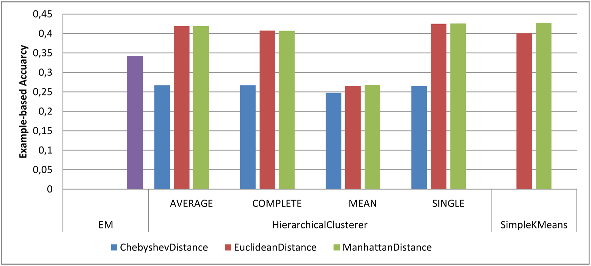
\includegraphics{figures/cml_cluster.pdf}
					\caption{Average Example-based accuracy for different cluster algorithm on CML over different datasets}
					\label{fig:cml_clus}
				\end{figure}

				\begin{figure}
					\centering			
					\subfigure[\scriptsize{Example-based Accuracy}]{
						\label{fig:fcml_clus_acc}
						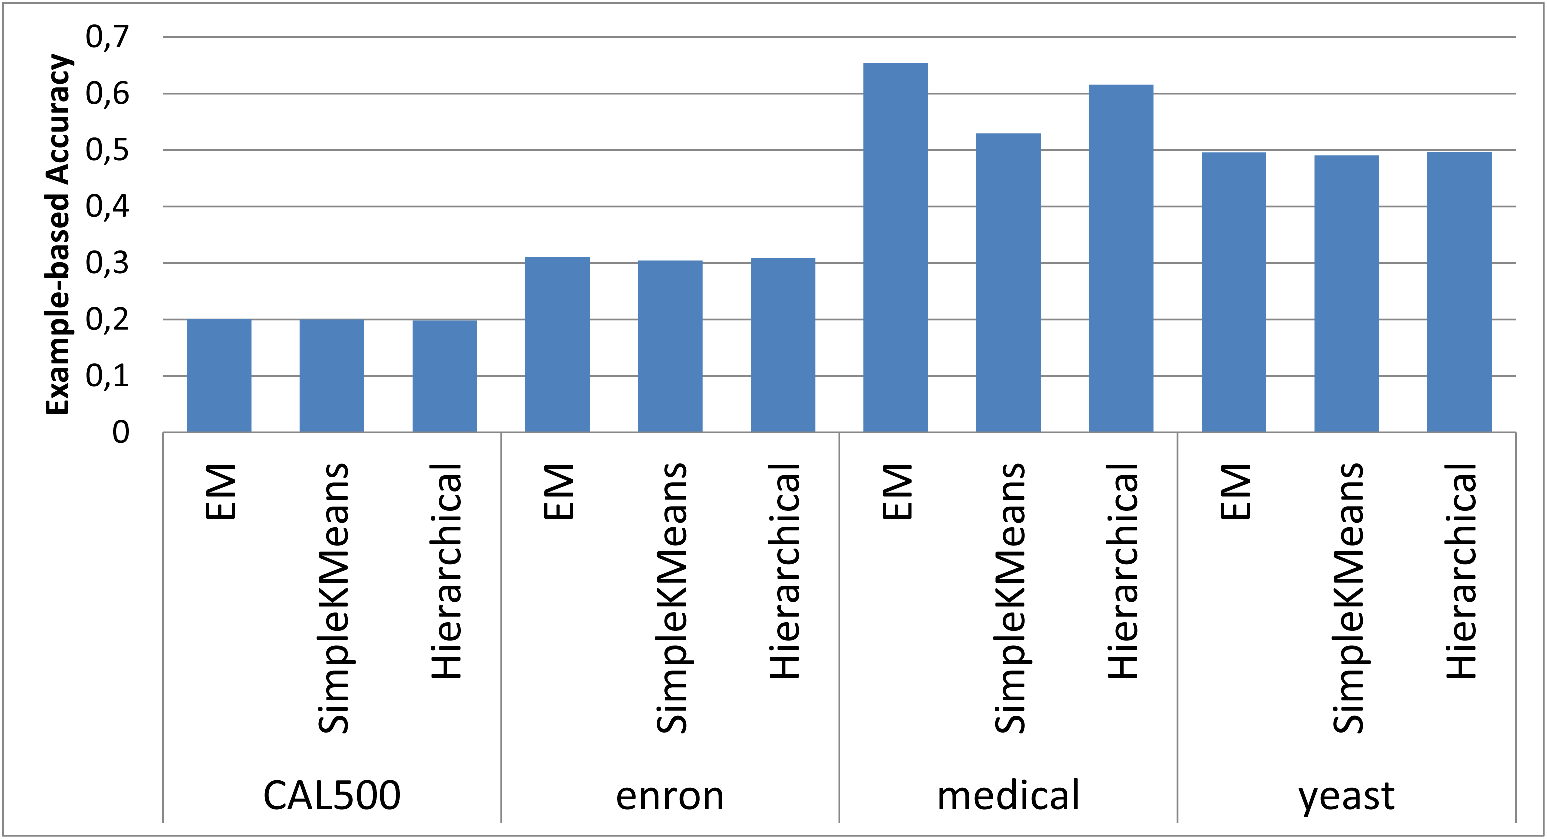
\includegraphics[width=.44\textwidth]{figures/fcml_cluster_acc.pdf}
					}
					\subfigure[\scriptsize{Micro-averaged F-Measure}]{
						\label{fig:fcml_clus_fmeasure}
						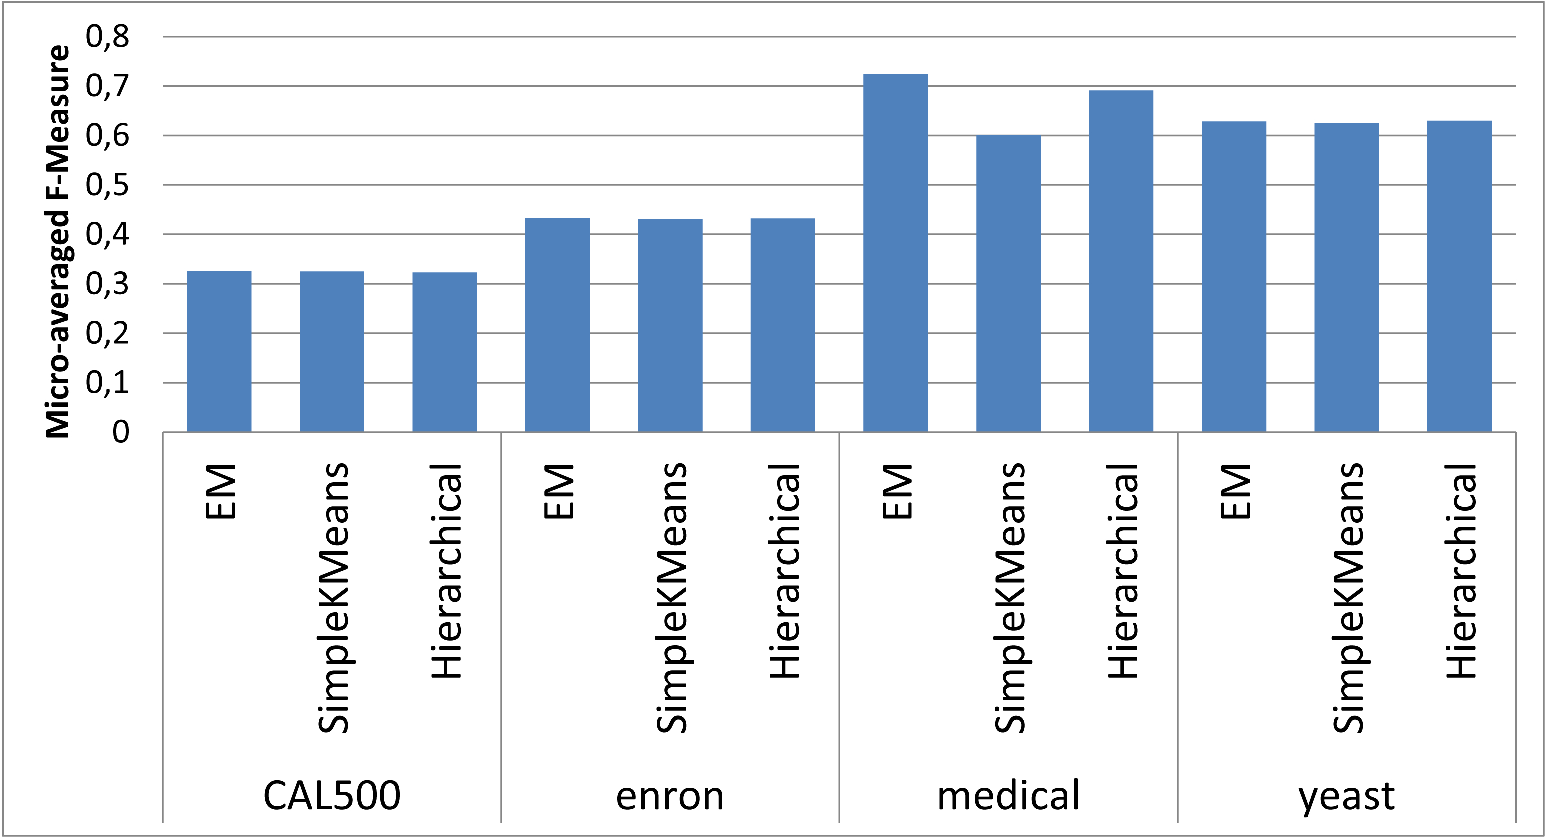
\includegraphics[width=.44\textwidth]	{figures/fcml_cluster_fmeasure.pdf}
					}
					\subfigure[\scriptsize{Hamming Loss}]{
						\label{fig:fcml_clus_hamming}
						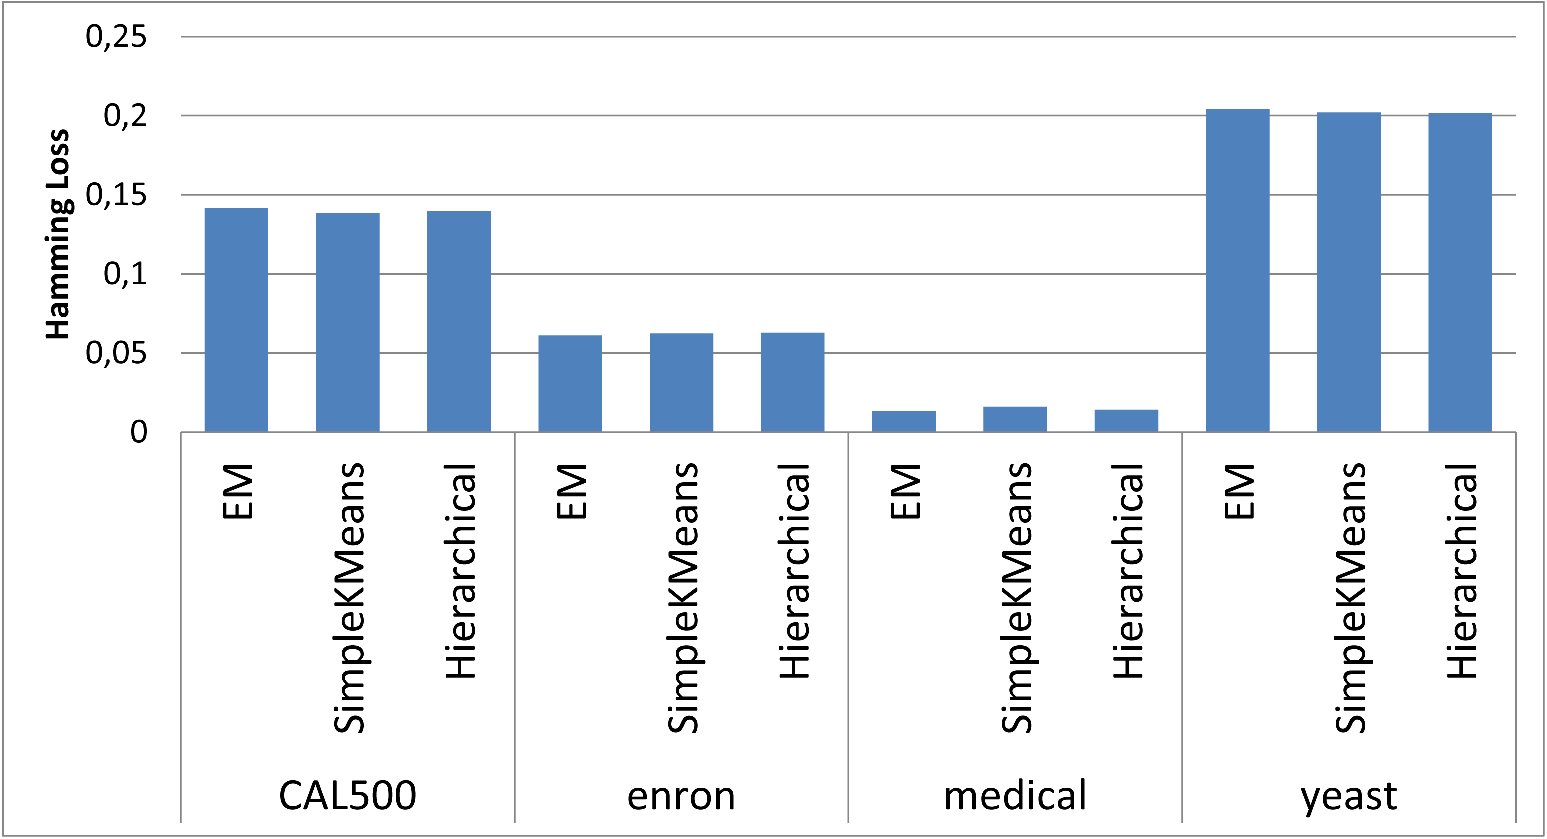
\includegraphics[width=.44\textwidth]{figures/fcml_cluster_hamming.pdf}
					}
					\caption{Evaluation of clustering algorithms in FCML. Different datasets were used. The measures are averaged over different settings, like $nc$, linkage criteria and distance measure}
					\label{fig:fcml_clus}
				\end{figure}

				\begin{figure}
					\centering			
					\subfigure[\scriptsize{Example-based Accuracy}]{
						\label{fig:fcml_clus_meth_acc}
						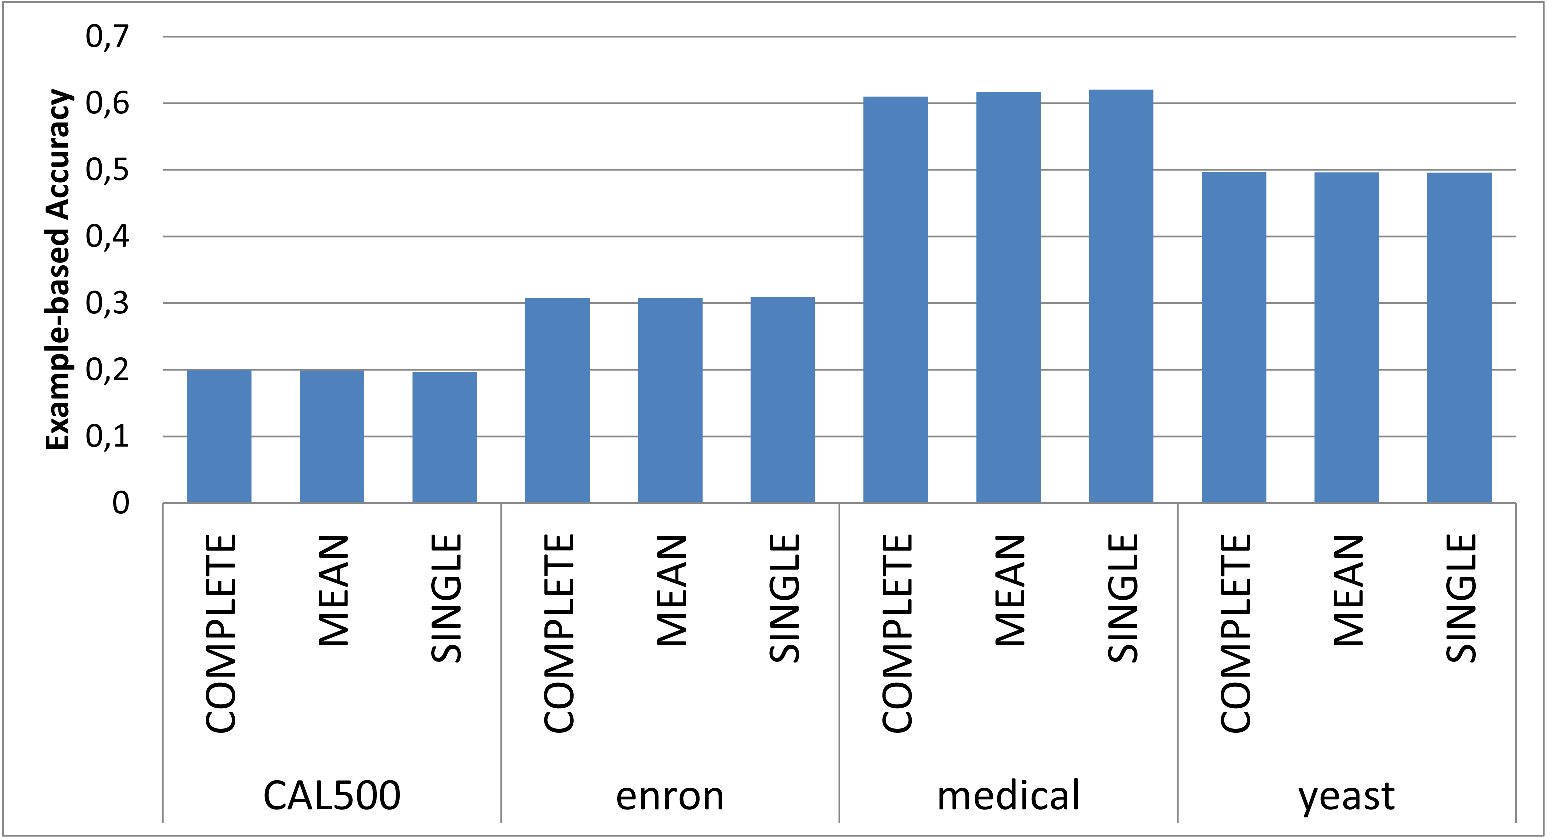
\includegraphics[width=.44\textwidth]{figures/fcml_clus_meth_acc.pdf}
					}
					\subfigure[\scriptsize{Micro-averaged F-Measure}]{
						\label{fig:fcml_clus_meth_fmeasure}
						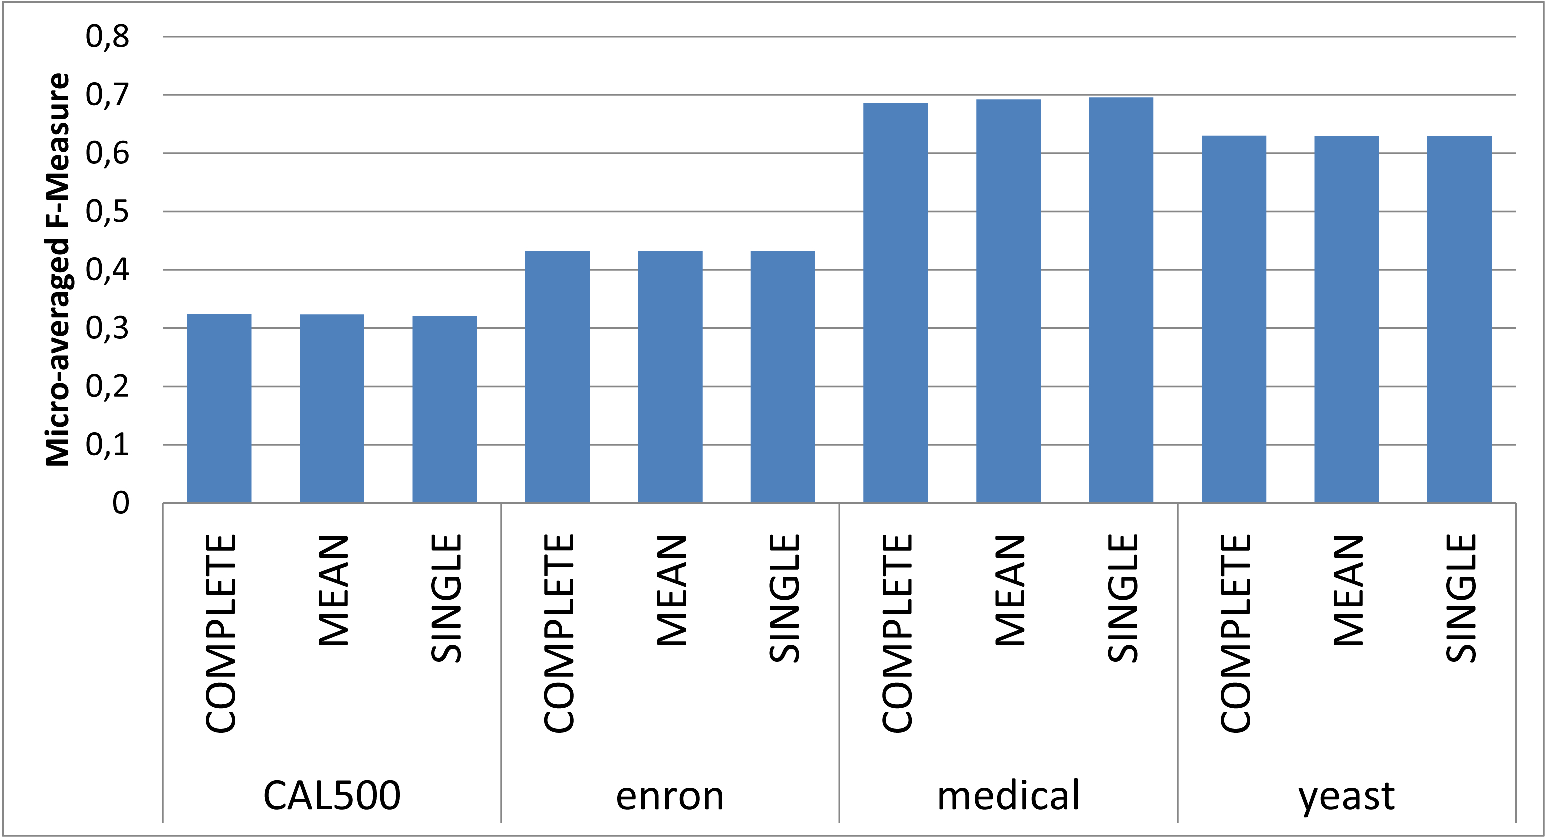
\includegraphics[width=.44\textwidth]	{figures/fcml_clus_meth_fmeasure.pdf}
					}
					\subfigure[\scriptsize{Hamming Loss}]{
						\label{fig:fcml_clus_meth_hamming}
						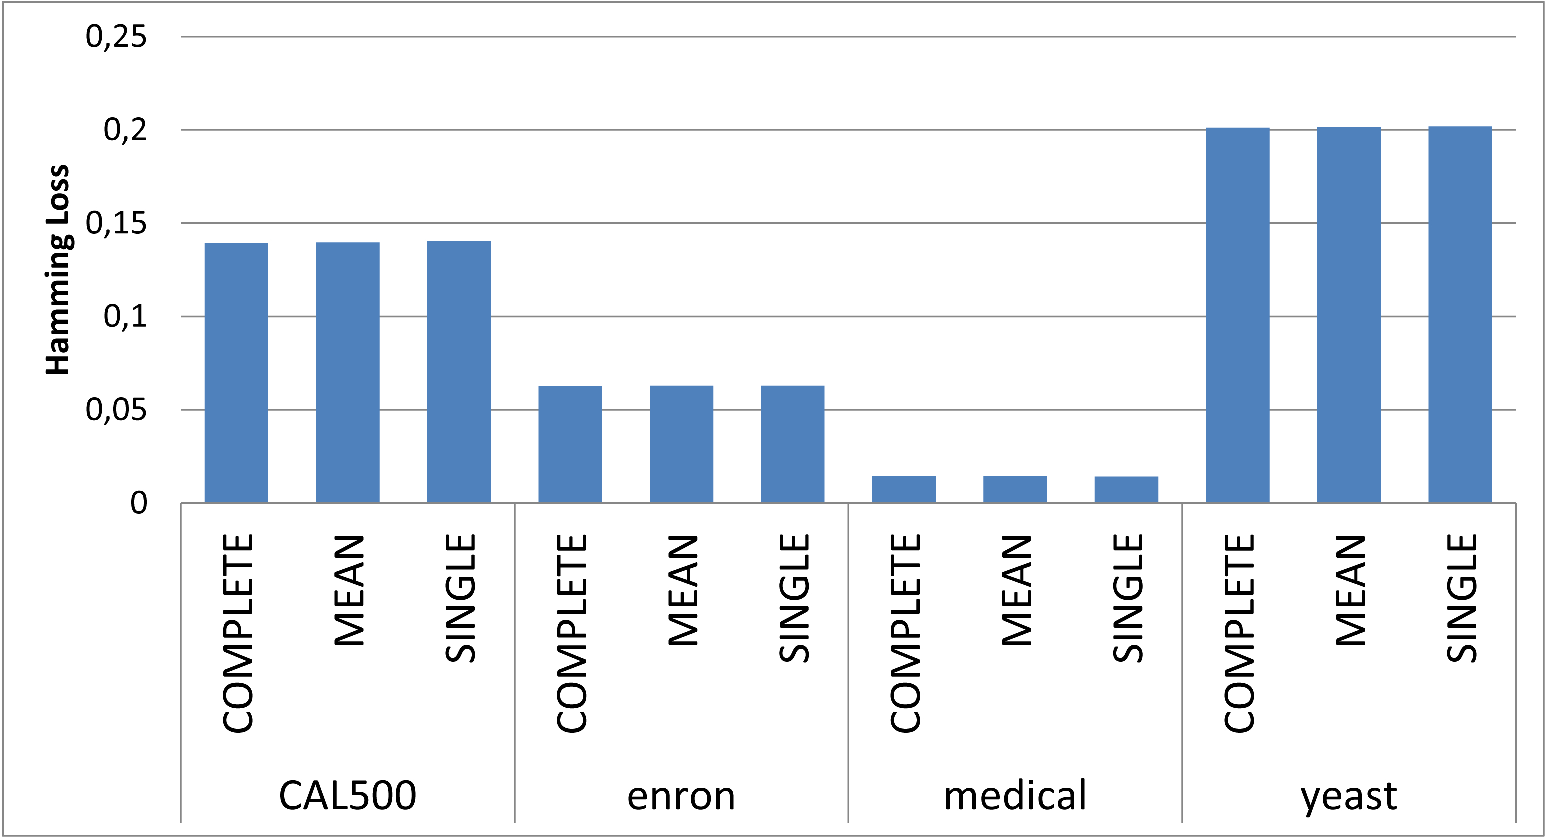
\includegraphics[width=.44\textwidth]{figures/fcml_clus_meth_hamming.pdf}
					}
					\caption{Evaluation of hierarchical clustering methods on different datasets. The measures are averaged over different distance measures}
					\label{fig:fcml_clus_meth}
				\end{figure}
					
				\begin{figure}
					\centering			
					\subfigure[\scriptsize{Example-based Accuracy}]{
						\label{fig:fcml_clus_dist_acc}
						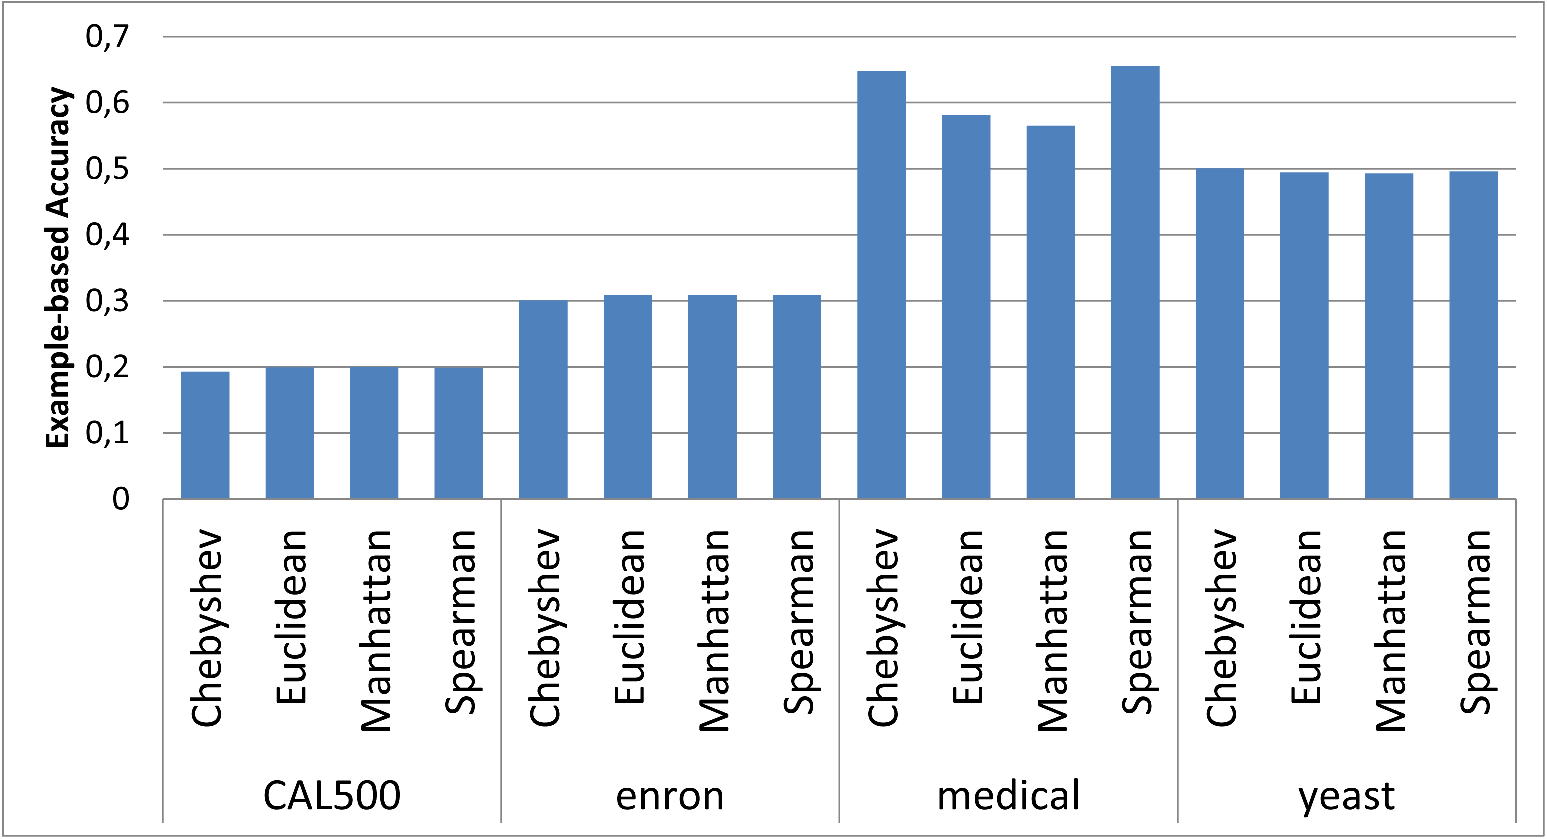
\includegraphics[width=.44\textwidth]{figures/fcml_clus_dist_acc.pdf}
					}
					\subfigure[\scriptsize{Micro-averaged F-Measure}]{
						\label{fig:fcml_clus_dist_fmeasure}
						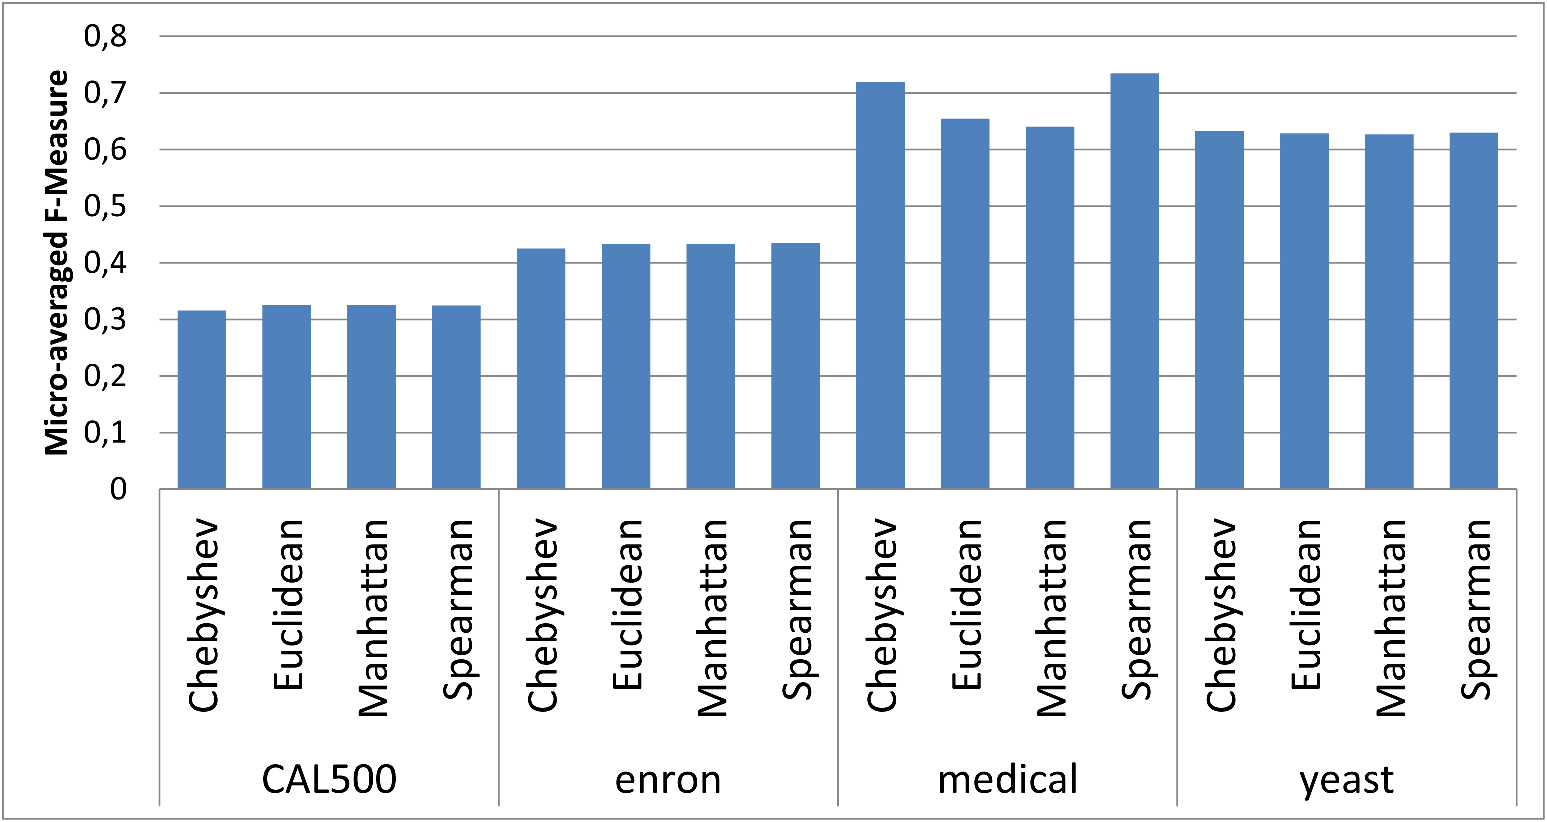
\includegraphics[width=.44\textwidth]	{figures/fcml_clus_dist_fmeasure.pdf}
					}
					\subfigure[\scriptsize{Hamming Loss}]{
						\label{fig:fcml_clus_dist_hamming}
						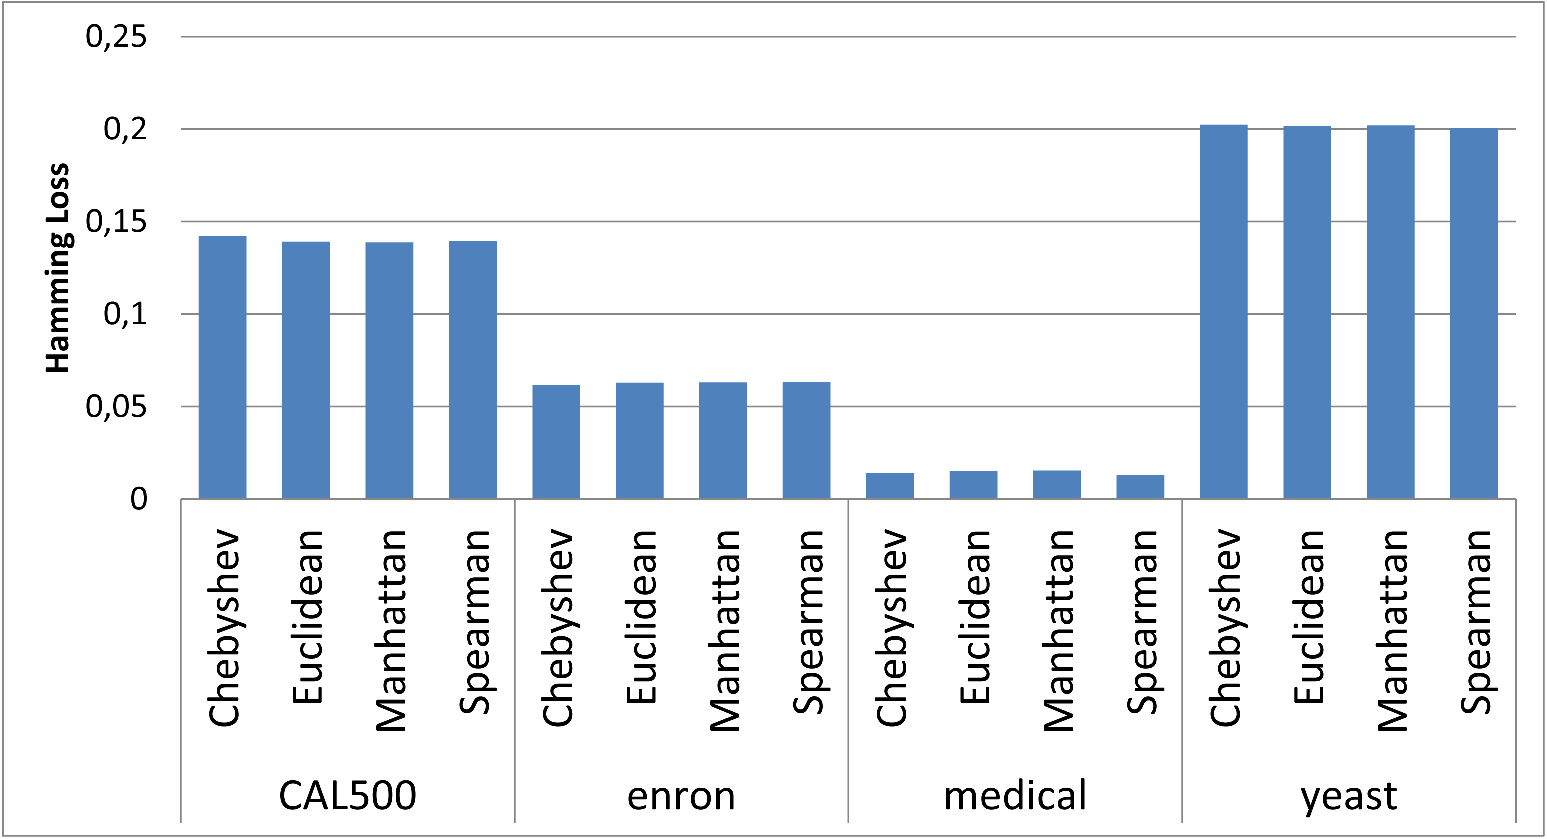
\includegraphics[width=.44\textwidth]{figures/fcml_clus_dist_hamming.pdf}
					}
					\caption{Evaluation of distance measure using hierarchical clustering on different datasets. The measures are averaged over different distance measures}
					\label{fig:fcml_clus_dist}
				\end{figure}


				\paragraph*{Number of clusters} Finally the parameter "number of clusters" has to be identified. The number of clusters ($nc$) can range from at least 2 to $|L|$, which results in each label to be clustered in a single cluster. Therefore, $nc$ is highly related to the size of the dataset, where $|L|$ can be between 14 (\textit{yeast}) and 983 (\textit{delicious}).

				For finding rules for determining $nc$, several attempts to identify correlations between $nc$ and evaluation measures like \textit{accuracy} or dataset specific measures like \textit{label-density} were made. Figure \ref{fig:clu_cor} shows the result for the setting "ClassifierChain, Hierarchical Clustering, single-linkage, Euclidean Distance, InformationGain" on the dataset \textit{CAL500}.
					
				In table \ref{tab:cor} a correlation matrix between the measures \textit{Example-based Accuracy}, \textit{Micro-averaged F-Measure}, \textit{Hamming-Loss} and \textit{avgDensity} as well the average labels per cluster and the number of clusters itself is shown. \textit{avgDensity} is the density averaged over all groups. The correlation was computed from the values for each step for $nc$ from 2 to $|L|$.
					
				The matrix shows poor correlation, with an exception on "Hamming-Loss" to "avgDensity". As the best value in Hamming-Loss is 0, performance seems to decrease with higher average density. However, the reason for this relationship could not be covered in this work due to time limits.
 
				\begin{figure}
					\centering
					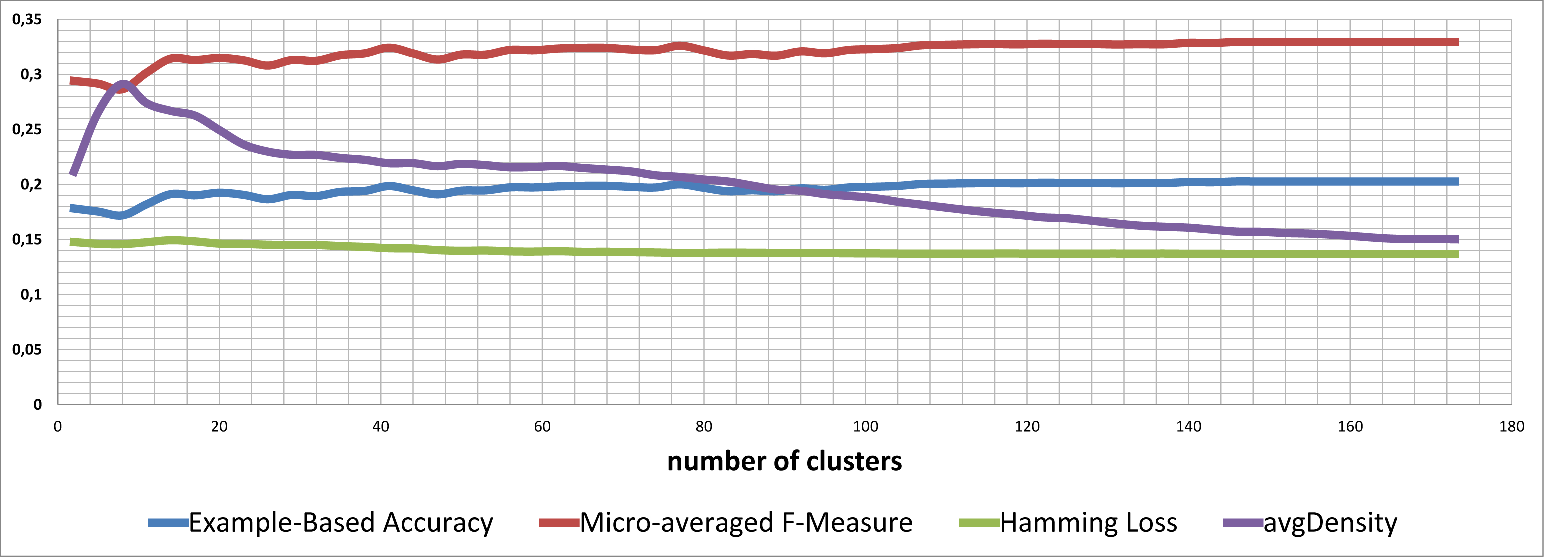
\includegraphics[width=.9\textwidth]{figures/cluster_corl.pdf}
					\caption{Example-based Accuracy, Micro-averaged F-Measure, Hamming Loss and average Density with growing number of clusters. The setting "ClassifierChain, Hierarchical Clustering, single-linkage, Euclidean Distance, InformationGain" \textit{CAL500} is used}
					\label{fig:clu_cor}
				\end{figure}

				\begin{table}\scriptsize
					\centering
					\begin{tabular}{r||r|r|r}
						& density & labels per cluster & number of clusters \\\hline\hline
						Accuracy & -0,2623 & -0,195886517 & -0,4528997 \\\hline
						F-Measure & -0,214 & -0,208032488 & -0,47366346 \\\hline
						HammingLoss & 0,78642 & 0,063797033 & 0,23463825 \\
					\end{tabular}
					\caption{Pearson-correlation matrix for the setting "ClassifierChain, Hierarchical Clustering, single-linkage, Euclidean Distance, InformationGain" \textit{CAL500} dataset with different $nc$}
					\label{tab:cor}
				\end{table}

		\subsection{Feature-Selection}

		FCML (see section \ref{sec:FCML}) uses feature selection methods to compute scores/ranks for every attribute. The configuration of the feature selection scenario is crucial to the learning and prediction process. 

		In order to isolate effects of ranking, in detail to ignore scores within the adding features to groups, any threshold is set to minimum. This leads to groups which only differ in the label subsets but always contain the entire features space. The evaluation of an optimal feature selection threshold is a separate task.
		
		To evaluate the feature selection process, a clustering algorithm is needed. To reduce the influence of good or bad clustering, various cluster algorithms and parameters were used. Finally, the performance of the FCML method is averaged.

		To reduce the number of evaluations, two scenarios where considered: Firstly, five feature selection methods were evaluated on one dataset, namely \textit{CAL500}. The results are shown in \ref{fig:fscal}. Although \textit{CfsSubsetEval} shows tiny improvements against other methods, no superior method could be determined.

		A second step evaluates three different feature selection methods on varying datasets: \textit{Relief}, \textit{CFS} and \textit{Information Gain}. Those three methods were chosen because they represent independent solution approaches. Results, as shown in figure \ref{fig:fs}, point out that CFS can outvalue both other methods only in the \textit{medical} dataset. Hence, Hamming-Loss shows no improvement.

		As no superior feature selection method could be found, further evaluation \textit{information gain} uses because of its simplicity. It computes mutual certainty for a pair of attributes satisfying the claim that groups consist of attributes which have strong mutual associations.
				
		\textit{Information gain} has also advantages in terms of computing time. Therefore, it allows more settings to be evaluated. Nevertheless, further evaluating and parameter optimization could lead to better results on certain datasets.

		\begin{figure}
			\centering
			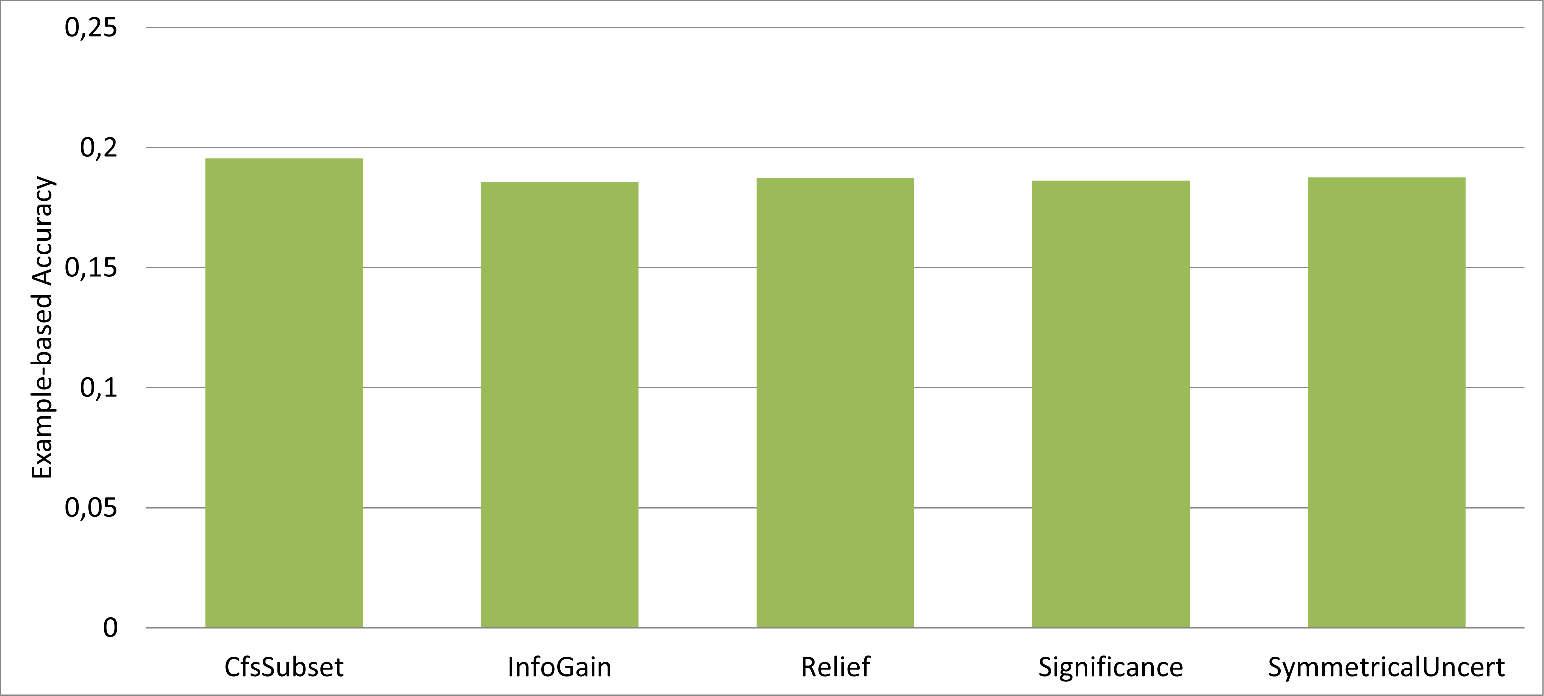
\includegraphics[width=.9\textwidth]{figures/five_fs.pdf}
			\caption{Feature-Selection Methods on the \textit{CAL500} dataset. Example-based Accuracy is averaged over different clustering settings}
			\label{fig:fscal}
		\end{figure}
				
		\begin{figure}
			\centering			
			\subfigure[\scriptsize{Example-based Accuracy}]{
				\label{fig:fcml_fs_acc}
				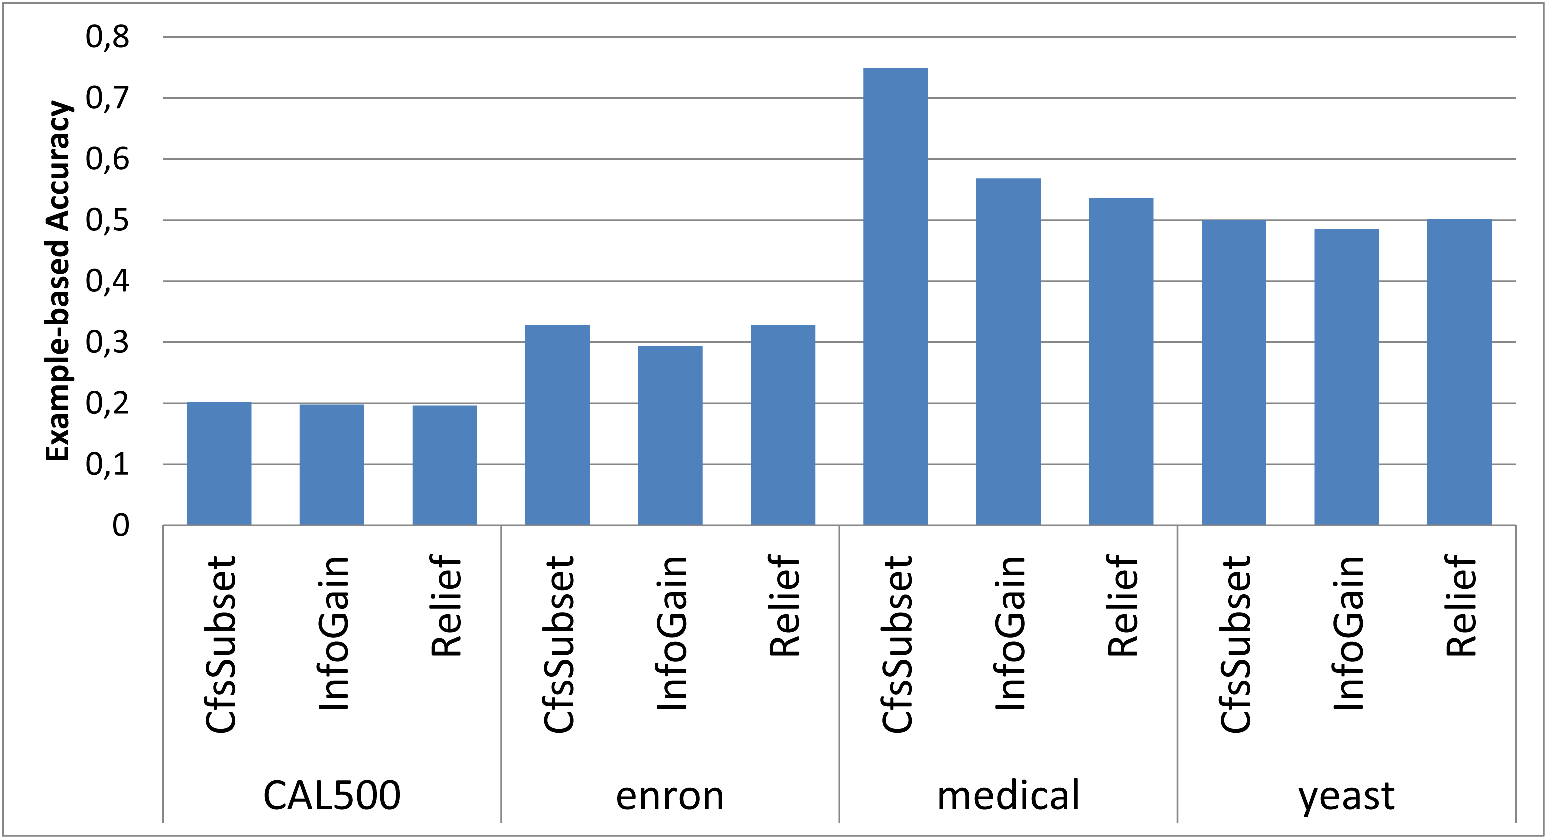
\includegraphics[width=.44\textwidth]{figures/fcml_fs_acc.pdf}
			}
			\subfigure[\scriptsize{Micro-averaged F-Measure}]{
				\label{fig:fcml_fs_fmeasure}
				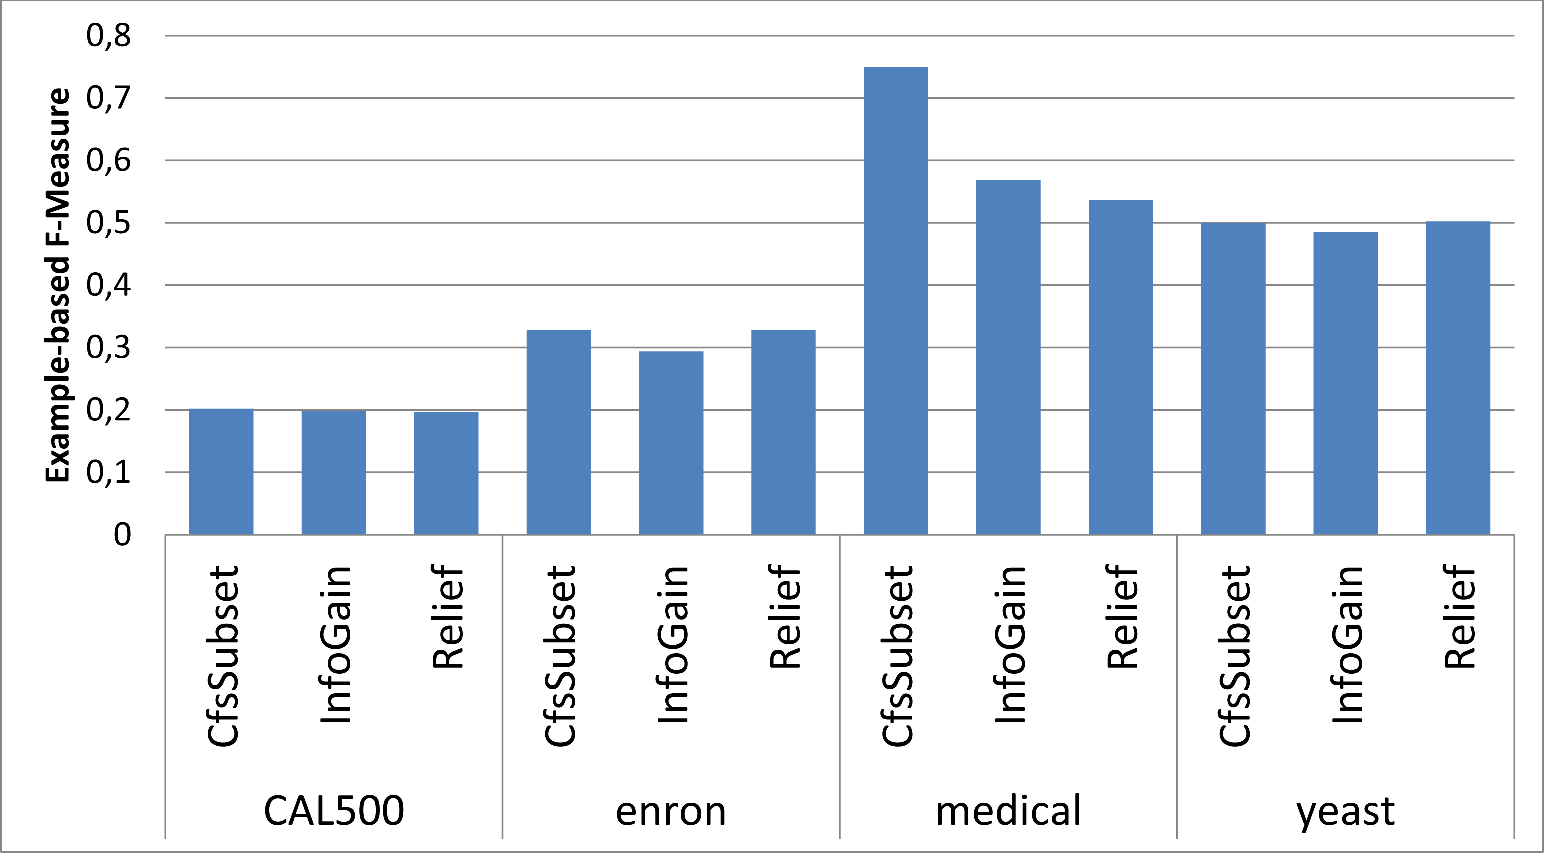
\includegraphics[width=.44\textwidth]	{figures/fcml_fs_fmeasure.pdf}
			}
			\subfigure[\scriptsize{Hamming Loss}]{
				\label{fig:fcml_fs_hamming}
				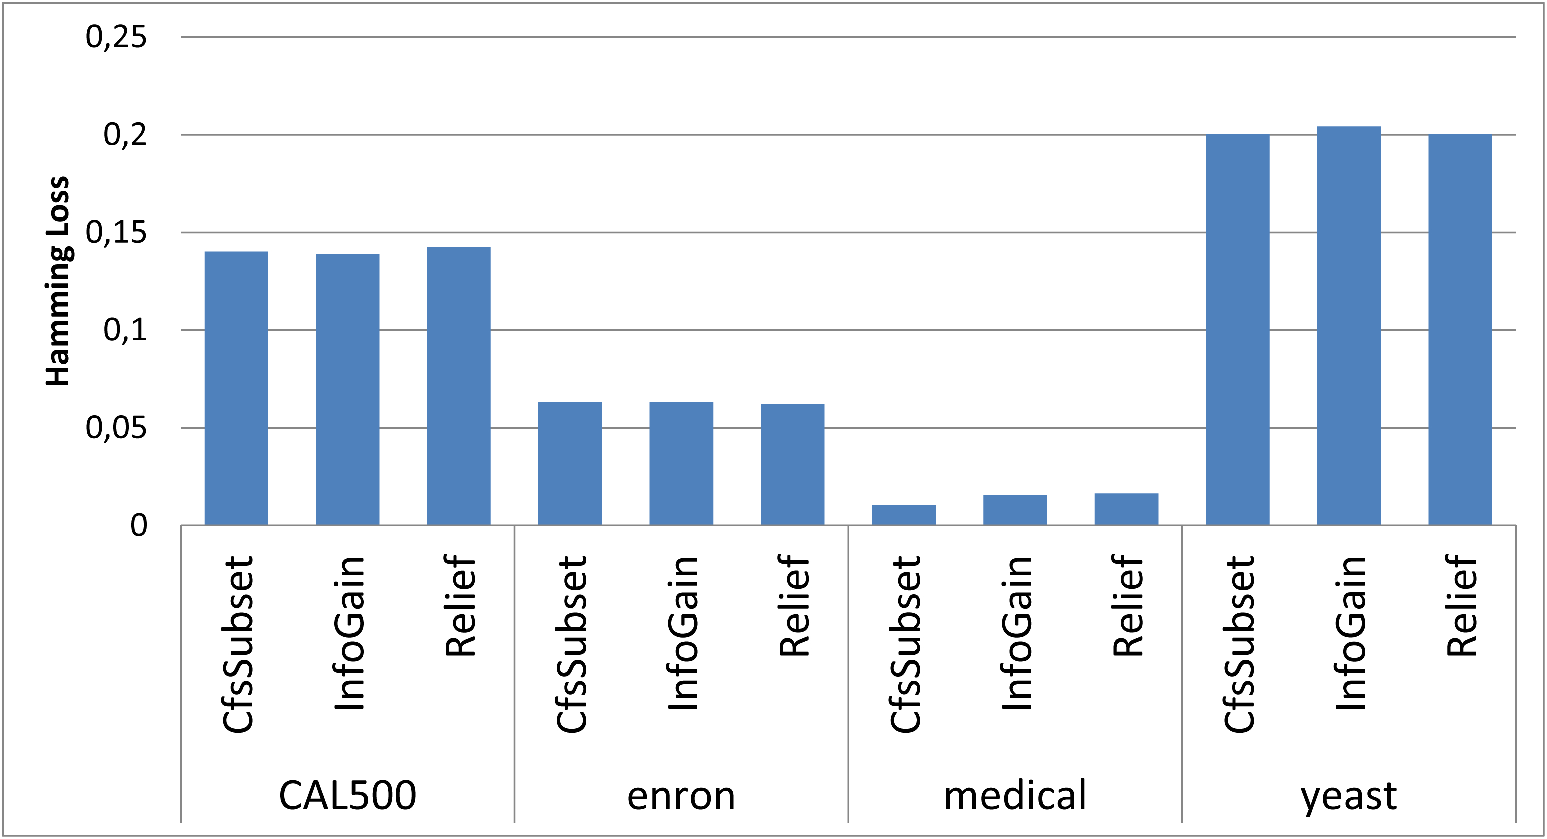
\includegraphics[width=.44\textwidth]{figures/fcml_fs_hamming.pdf}
			}
			\caption{\textit{Relief}, \textit{CFS} and \textit{Information Gain} feature selection on different datasets}
			\label{fig:fs}
		\end{figure}

	\subsection{Evaluation of methods}

		In the following, results from CML and FCML are presented. Note that CML was developed and tested prior to FCML, the latter one uses an extended set of datasets and evaluation techniques. Due to time limits it was not possible to repeat tests for CML with new datasets.

		\subsubsection{CML}

			\begin{figure}
				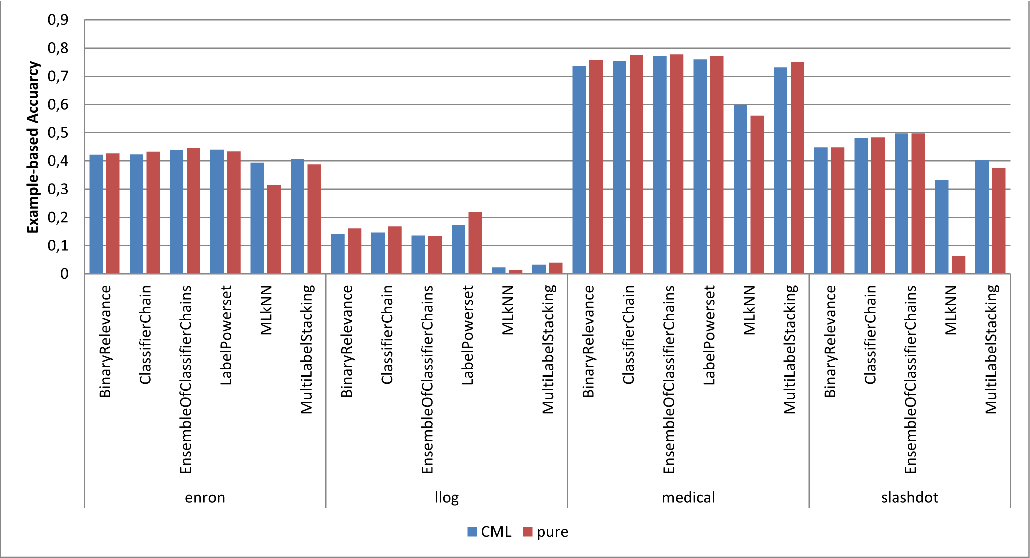
\includegraphics[width=\textwidth]{figures/cml_results.pdf}
				\caption{CML compared to pure multi-label learners using the example-based accuracy. For CML the best result is taken.}
				\label{fig:cml}
			\end{figure}

			In figure \ref{fig:fs} results of CML compared to pure multi-label learners are shown. If needed by the multi-label learner, a Support-Vector Machine (SMO) was used. As described before a hierarchical clustering with Euclidean distance measure and single-linkage was used. For the number of clusters, $nc$, different number of clusters, namely $2, 4, 6$, where chosen. For the results the best $nc$ was taken. All evaluation was done by a 5-fold cross-validation.

			Although nearly every scenario shows similar results for CML and the pure learner, performance of ML-kNN could be improved in every case.

			ML-kNN computes distances between instances and assigns query instance to the major label set of the k-nearest neighbors using a maximum-a-posteriori principle. Filtering the label space can enhance the MAP principle as the elements of the output label space are highly dependent and therefore MAP probabilities are likely to be high.

			In summery, CML can enhance the performance of multi-label learners in some cases, but on average CML shows the same performance as its pure multi-label scheme.

		\subsubsection{FCML}

			Results for FCML are shown in figure \ref{fig:fcml_res}. For every scenario (dataset + multi-label learner), all possible numbers of clusters $nc$ were evaluated and the best result is presented. To reduce the complexity of parameters, feature selection was used without threshold, e.g. groups always contain the entire feature space. HOMER, as described in section \ref{subsubsec:homer} was used for comparison. HOMER uses a parameter $k$ describing for the number of clusters at each hierarchical level. Every scenario, $k=2\hdots 8$ was evaluated and again the best result is presented. However, HOMER did not finish in every scenario due to memory limits (6GB) or problems in the implementation\footnote{IndexOutOfBounds-Exception during JAVA runtime}. In addition, for every scenario a pure multi-label learner has been trained.

			\begin{figure}
				\centering
				\subfigure[Example-based Accuracy]{
					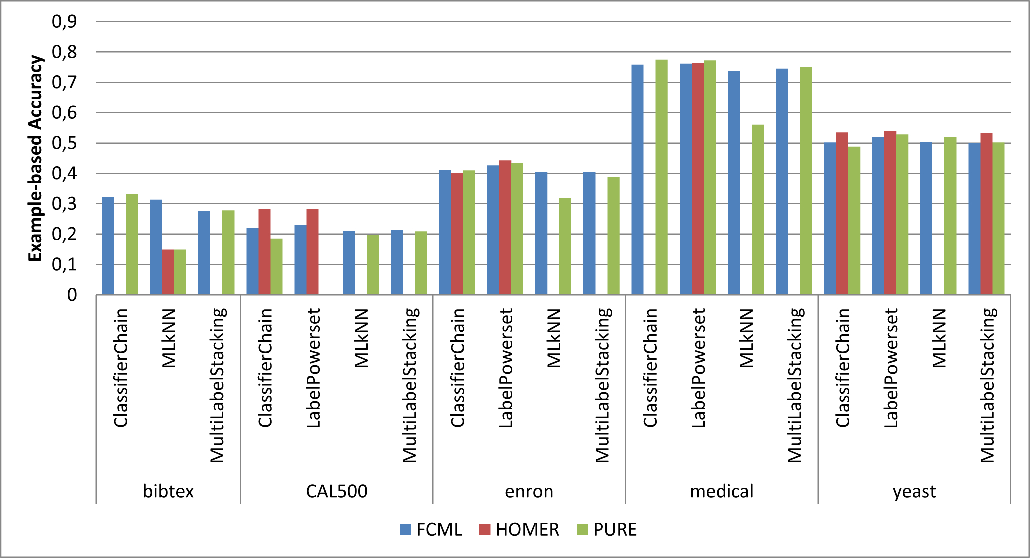
\includegraphics[width=.73\textwidth]{figures/fcml_acc.pdf}
				}
				\subfigure[Micro-averaged F-Measure]{
					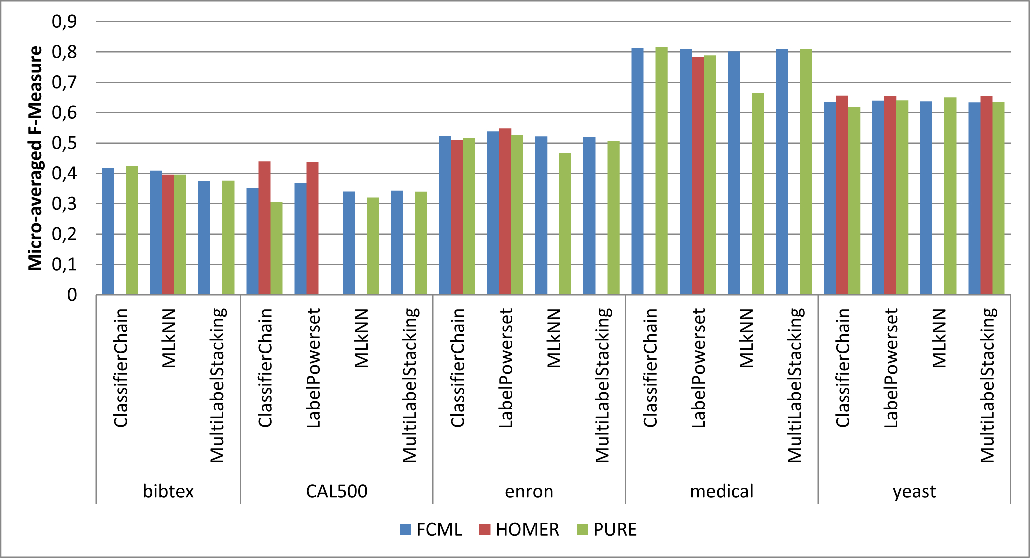
\includegraphics[width=.73\textwidth]{figures/fcml_fmeasure.pdf}
				}
				\subfigure[Hamming Loss]{
					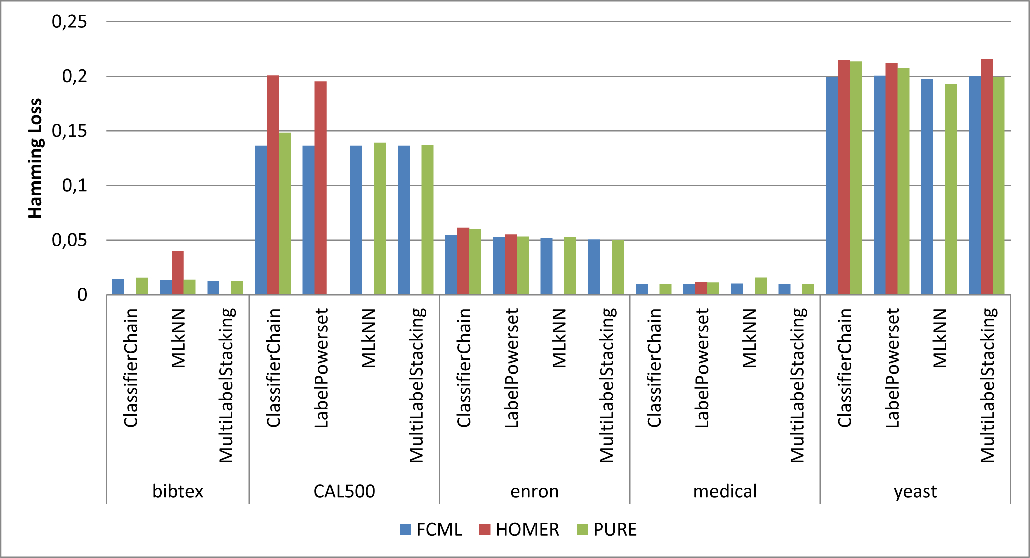
\includegraphics[width=.73\textwidth]{figures/fcml_hamming.pdf}
				}
				\caption{FCML compared to pure multi-label learners and HOMER on different datasets. In every setting the best result is presented. HOMER did not finish on all scenarios.}
				\label{fig:fcml_res}
			\end{figure}

			FCML does not show superior results in Example-based Accuracy. Merely Hamming Loss could be reduced in some cases. Still, ML-kNN could be enhanced in some cases: \textit{enron}, \textit{medical}, \textit{bibtex}. HOMER performs better in almost any case. Best results for FCML in this scenario are achieved with $nc=158$ being a clustering of every label into a sole cluster which indicates there are very few dependencies in the label space.

			In terms of Hamming Loss or Micro-Averaged F-Measure, FCML can achieve small enhancements to the pure and HOMER multi-label learner. Both Hamming Loss and Micro-Averaged F-Measure take false positives into account, while accuracy does not. That indicates that FCML has slightly better performance in predicting absent labels compared to pure and HOMER. By reducing the label space and therefore reducing the influences of other labels, non-relevant and misleading signals are eliminated.

			It is problem to identify the effect of $nc$ on the performance as different multi-label learners perform best on very different $nc$: For example the \textit{bibtext} dataset with $|L|=158$, where Classifier Chains have the best result with a $nc=8$, MlKNN $k=158$ and MultiLabel-Stacking with $nc=14$.

			\subsubsection{Summary}

				The results show that a clustering of labels into different groups and splitting the dataset according to those label sets does not cause a lower predicting performance. Even very strong splitting, where every label falls into a single cluster, may enhance the performance, what indicates that inter-label relations are not used. Prediction of absent labels could be slightly enhanced, indicated by lower Hamming Loss results. This is done by reducing the noise in the label-space by grouping them into smaller subsets.